%--------------------------------------------------------------------
\section{Core Vocabulary Overview}
\label{fresnelov}

Fresnel is an RDF vocabulary, described by an OWL ontology \cite{fresnel05}. Fresnel presentation knowledge is thus expressed declaratively in RDF and relies on two foundational concepts: {\em lenses} and {\em formats} (see Figure \ref{foundationalConceptsFig}). Lenses specify which properties of RDF resources are shown and how these properties are ordered while formats indicate how to format content selected by lenses and optionally generate additional static content and hooks in the form of CSS class names that can be used to style the output through external CSS style sheets. The following sections introduce the main vocabulary elements using the examples in Figures \ref{exampleFig} and \ref{exampleFig2}.

\begin{figure}
\begin{center}
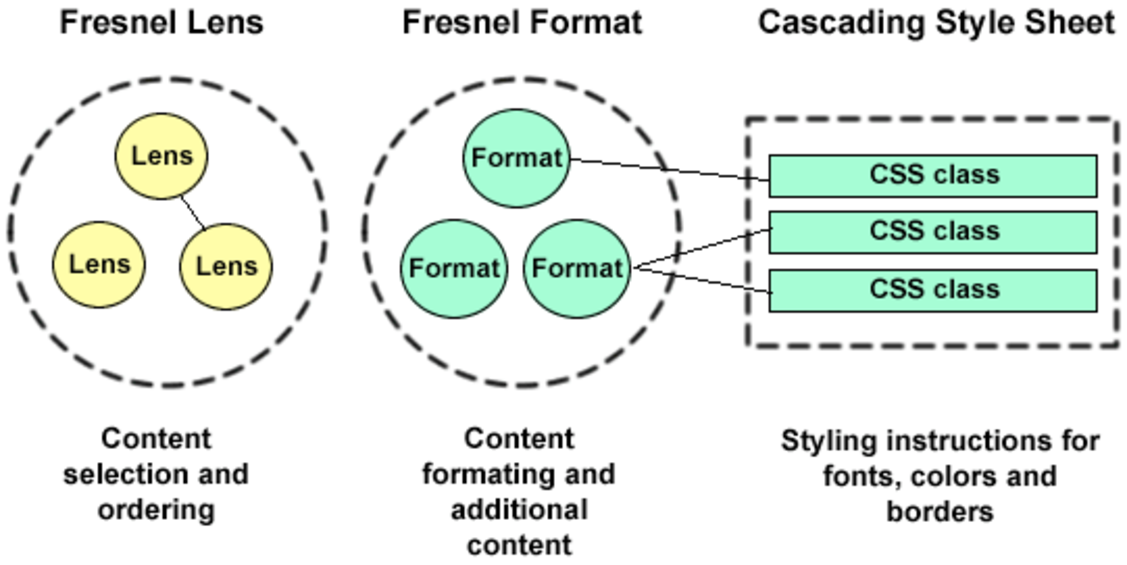
\includegraphics[width=10cm]{overview.pdf}
\caption{Fresnel foundational concepts}
\label{foundationalConceptsFig}
\end{center}
\end{figure}

Figure \ref{exampleFig} shows a simple lens and associated formats used to present information about a person described with the FOAF vocabulary \cite{foaf}. This figure also shows a possible rendering of such a resource, that a browser like Horus~\cite{horus} or Longwell~\cite{simile} could produce. Examples use the Notation 3 syntax \cite{N3}.

\begin{figure}
\begin{tabular}{lp{4.5cm}}
\begin{small}
\begin{tabular}{ll}
(300) & \rdf{ :PersonLens a fresnel:Lens ;} \\
(301) & \rdf{ ~fresnel:classLensDomain foaf:Person ;} \\
(302) & \rdf{ ~fresnel:showProperties (} \\
(303) & \rdf{ ~~foaf:name} \\
(304) & \rdf{ ~~foaf:mbox} \\
(305) & \rdf{ ~~[rdf:type fresnel:PropertyDescription;} \\
(306) & \rdf{ ~~~fresnel:alternateProperties (} \\
(307) & \rdf{ ~~~   foaf:depiction foaf:img p3p:image )} \\
(308) & \rdf{ ~~~] ) .} \\
 & \\
(309) & \rdf{ :nameFormat a fresnel:Format ; } \\
(310) & \rdf{ ~~~~fresnel:propertyFormatDomain foaf:name ;} \\
(311) & \rdf{ ~~~~fresnel:label "Name" .} \\
 & \\
(312) & \rdf{ :mboxFormat a fresnel:Format ;} \\
(313) & \rdf{ ~~~~fresnel:propertyFormatDomain foaf:mbox ;} \\
(314) & \rdf{ ~~~~fresnel:label "Mailbox" ;} \\
(315) & \rdf{ ~~~~fresnel:value fresnel:externalLink ;} \\
(316) & \rdf{ ~~~~fresnel:valueFormat [ fresnel:contentAfter "," ] .} \\
 & \\
(317) & \rdf{ :depictFormat a fresnel:Format ;} \\
(318) & \rdf{ ~~~~fresnel:propertyFormatDomain foaf:depiction ;} \\
(319) & \rdf{ ~~~~fresnel:label fresnel:none ;} \\
(320) & \rdf{ ~~~~fresnel:value fresnel:image .} \\
\end{tabular}
\end{small}
&
\begin{picture}(45,0.1)(0,0)\put(-26,67){\makebox(0,0){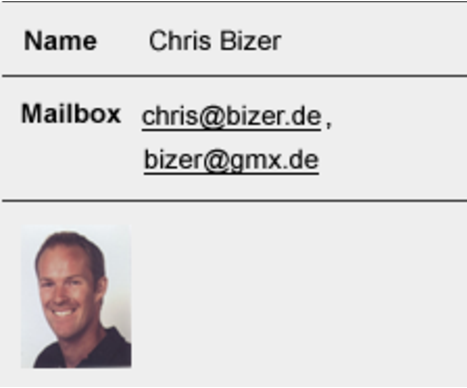
\includegraphics[width=4cm]{boxmodelexampleoutput.pdf}}}\end{picture} \\
\end{tabular}
\caption{A lens and some formats for presenting instances of class \rdf{foaf:Person}}
\label{exampleFig}
\vspace{-2em}
\end{figure}

\subsection{Content selection}

The domain of a lens indicates the set of resources to which a lens applies (line 301: the lens applies to instances of class \rdf{foaf:Person}). Property \rdf{fresnel:showProperties} is used to specify what properties of these resources to show and in what order (lines 302-308). In this example, the values of both \rdf{fresnel:classLensDomain} and \rdf{fres\-nel:showProperties} are basic selectors, which take the form of plain URIs (represented here as qualified names), respectively identifying the class of resources and property types to select. More advanced selection expressions can be written using either FSL or SPARQL. They make it possible to associate lenses with untyped RDF resources, which do occur in real-world models since \rdf{rdf:type} properties are not mandatory. They can also be used to specify that a lens should display all properties of a given namespace, or any other complex selection condition(s) that can be represented by an FSL or SPARQL expression (see Section \ref{selectors}).

Fresnel Core provides additional constructs for specifying what properties of resources to display. The special value \rdf{fresnel:allProperties} is used when the list of properties that can potentially be associated with resources handled by a lens is unknown to the lens' author but should nevertheless be displayed. When it appears as a member of the list of properties to be shown by a lens, \rdf{fresnel:allProperties} designates the set of properties that are not explicitly designated by other property URI references in the list, except for properties that appear in the list of properties to hide (\rdf{fresnel:hideProperties}). Two other constructs are used to handle the potential irregularity of RDF data stemming from the fact that different authors might use similar terms coming from different vocabularies to make equivalent statements. Sets of such similar properties can be said to be \rdf{fresnel:alternateProperties}. For instance, \rdf{foaf:depiction}, \rdf{foaf:img} and \rdf{p3p:image} could be considered as providing the same information about resources displayed by a given lens. A browser using this lens would try to display the resource's \rdf{foaf:depiction}. If the latter did not exist, the browser would then look for \rdf{foaf:img} or \rdf{p3p:image} (see lines 305-307). Such knowledge can also be represented through ontology mapping mechanisms, but Fresnel provides this alternative as the ontology layer should not be made a requirement of the Fresnel presentation process. The other construct, \rdf{fresnel:mergeProperties}, is used to merge the values of related properties (e.g. \rdf{foaf:homepage} and \rdf{foaf:work\-Homepage}) into one single set of values that can later be formatted as a whole. 

The presentation of property values is not limited to a single level, and (possibly recursive) calls to lenses can be made to display details about the value of a property. Lenses used in this context are referred to as {\em sublenses}. Modifying the example of Figure \ref{exampleFig}, we specify in Figure \ref{exampleFig2} that the browser should render values of the property \rdf{foaf:knows} (lines 405-407) using another lens (\rdf{PersonLabelLens}, lines 410-413). The FSL expression (see Section \ref{selectors}) on line 406 specifies in an XPath-like manner that only values of \rdf{foaf:knows} that are instances of \rdf{foaf:Person} should be selected.

The sublens mechanism implies that a lens can recursively call itself as a sublens for displaying property values. In order to prevent infinite loops caused by such recursive calls, Fresnel defines a closure mechanism that allows Fresnel presentation designers to specify the maximum depth of the recursion.

\subsection{Content formatting}

The default layout of selected information items is highly dependent on the browser's representation paradigm (e.g. nested box layout, node-link diagrams, etc.), but the final rendering can be customized by associating formatting and styling instructions with elements of the representation.

\begin{picture}(340,1)(0,-5)
  \put(-10,0){\line(1,0){340}}
\end{picture}
\begin{figure}
\vspace{-4em}
\begin{tabular}{lp{4.5cm}}
\begin{small}
\begin{tabular}{ll}
(400) & \rdf{:PersonLens a fresnel:Lens ;}\\
(401) & \rdf{ ~~fresnel:classLensDomain foaf:Person ;} \\
(402) & \rdf{ ~~fresnel:showProperties (} \\
(403) & \rdf{ ~~~~foaf:name} \\
(404) & \rdf{ ~~~~foaf:mbox} \\
(405) & \rdf{ ~~~~[rdf:type fresnel:PropertyDescription ;} \\
(406) & \rdf{ ~~~~~fresnel:property "foaf:knows[foaf:Person]"}\srdf{$^{\wedge\wedge}$fresnel:fslSelector;} \\
(407) & \rdf{ ~~~~~fresnel:sublens :PersonLabelLens] } \\
(408) & \rdf{ ~~) ;} \\
(409) & \rdf{ ~~fresnel:group :FOAFmainGroup .} \\
 & \\
(410) & \rdf{ :PersonLabelLens a fresnel:Lens ;} \\
(411) & \rdf{ ~~fresnel:classLensDomain foaf:Person ;} \\
(412) & \rdf{ ~~fresnel:showProperties ( foaf:name ) ;} \\
(413) & \rdf{ ~~fresnel:group :FOAFsubGroup .} \\
 & \\
(414) & \rdf{ :nameFormat a fresnel:Format ; } \\
(415) & \rdf{ ~~fresnel:propertyFormatDomain foaf:name ;} \\
(416) & \rdf{ ~~fresnel:label "Name" ;} \\
(417) & \rdf{ ~~fresnel:group :FOAFmainGroup .} \\
 & \\
(418) & \rdf{ :mboxFormat a fresnel:Format ;} \\
(419) & \rdf{ ~~fresnel:propertyFormatDomain foaf:mbox ;} \\
(420) & \rdf{ ~~fresnel:label "Mailbox" ;} \\
(421) & \rdf{ ~~fresnel:value fresnel:externalLink ;} \\
(422) & \rdf{ ~~fresnel:valueFormat [ fresnel:contentAfter "," ] ;} \\
(423) & \rdf{ ~~fresnel:group :FOAFmainGroup .} \\
 & \\
(424) & \rdf{ :friendsFormat a fresnel:Format ;} \\
(425) & \rdf{ ~~fresnel:propertyFormatDomain foaf:name ;} \\
(426) & \rdf{ ~~fresnel:label "Friends" ;} \\
(427) & \rdf{ ~~fresnel:group :FOAFsubGroup .} \\
 & \\
(428) & \rdf{ :FOAFmainGroup a fresnel:Group .} \\
(429) & \rdf{ :FOAFsubGroup a fresnel:Group .} \\
 \end{tabular}
\end{small}
&
\begin{picture}(45,10)(0,0)\put(-73,60){\makebox(0,0){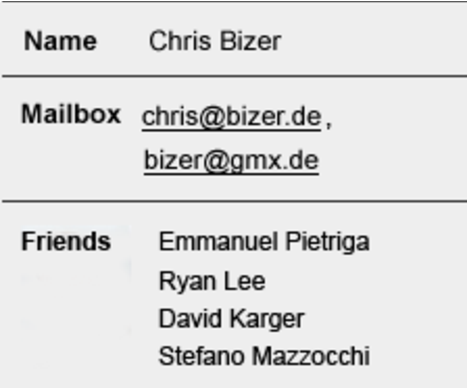
\includegraphics[width=4.2cm]{boxmodelexampleoutput2.pdf}}}\end{picture} \\
\end{tabular}
\caption{An example of a lens using another lens to display some property values}
\label{exampleFig2}
\vspace{-2em}
\end{figure}

\begin{picture}(340,1)(0,-10)
  \put(-10,0){\line(1,0){340}}
\end{picture}

Formats apply to resources, or to properties and their values, depending on the specified domain. The three example formats of Figure \ref{exampleFig} apply respectively to the properties \rdf{foaf:name}, \rdf{foaf:mbox} and \rdf{foaf:depiction} (lines 310, 313, 318). Formats can be used to set properties' labels (lines 311, 314, 319). Property \rdf{fresnel:label} does not specify a particular layout but simply gives a text string that can be used to identify the property. Labels might already be defined for many properties (e.g., in the associated vocabulary description using \rdf{rdfs:label}), but such labels are not guaranteed to exist. Moreover, a given label might not always be the most appropriate depending on the context in which the property is displayed. For instance, the default label associated with property \rdf{foaf:name} in the FOAF schema is {\em name}. When displaying the persons known by the current person in Figure \ref{exampleFig2}, this default label is replaced by {\em Friends} (line 426) so as to indicate the appropriate interpretation of the corresponding \rdf{foaf:name} property values in this context. The customization of labels also proves useful when displaying property values that are not direct properties of the current resource, as is made possible by the use of SPARQL or FSL expressions such as:
\[ \rdf{foaf:knows/*[airport:iataCode/text() = 'CDG']/foaf:name} \]
which would require an explanatory label such as {\em Friends that leave near Paris}.

Formats can also give instructions regarding how to render values. For instance, line 315 indicates that \rdf{foaf:mbox} values should be rendered as clickable links (email addresses). Values of \rdf{foaf:depiction} should be fetched from the Web and rendered as bitmap images (line 320).

Property values can be grouped, and additional content such as commas and an ending period can be specified to present multi-valued properties (line 316: inserting a comma in-between each email address). CSS class names can also be associated with the various elements being formatted. These names appear in the output document and can be used to style the output by authoring and referencing CSS style sheets that use rules with the same class names as selectors.

\subsection{Lens and Format Grouping}

Lenses and formats can be associated through \rdf{fresnel:Group}s so that browsers can determine which lenses and formats work together.  Fresnel groups are taken into account by browsers when selecting what format(s) to apply to the data selected by a given lens, as several formats might be applicable to the same property values.

Figure \ref{exampleFig2} illustrates the use of Fresnel groups to display different labels for the \rdf{foaf:name} property depending on the context in which the property is shown: the property is labeled {\em Name} when displayed in the context of the \rdf{PersonLens} lens, but is labeled {\em Friends} when displayed in the context of the \rdf{PersonLabelLens} lens. This is achieved by associating the \rdf {PersonLens} (lines 400-409) and the \rdf{nameFormat} (lines 414-417) to one group: \rdf{FOAFmainGroup}, and by associating the \rdf{PersonLabelLens} (lines 410-413) and the \rdf{friendsFormat} (lines 424-427) to a second group: \rdf{FOAFsub\-Group}.

A Fresnel group can also serve as a placeholder for formatting instructions that apply to all formats associated with that group, thus making it possible to factorize the declarations. It is also typically used to declare group-wide data, relevant to both lenses and formats, such as namespace prefix bindings.
